% Tikz File 'pregel_trace.tex'
\documentclass{standalone}
\usepackage{tikz}
\usetikzlibrary{positioning}
\begin{document}
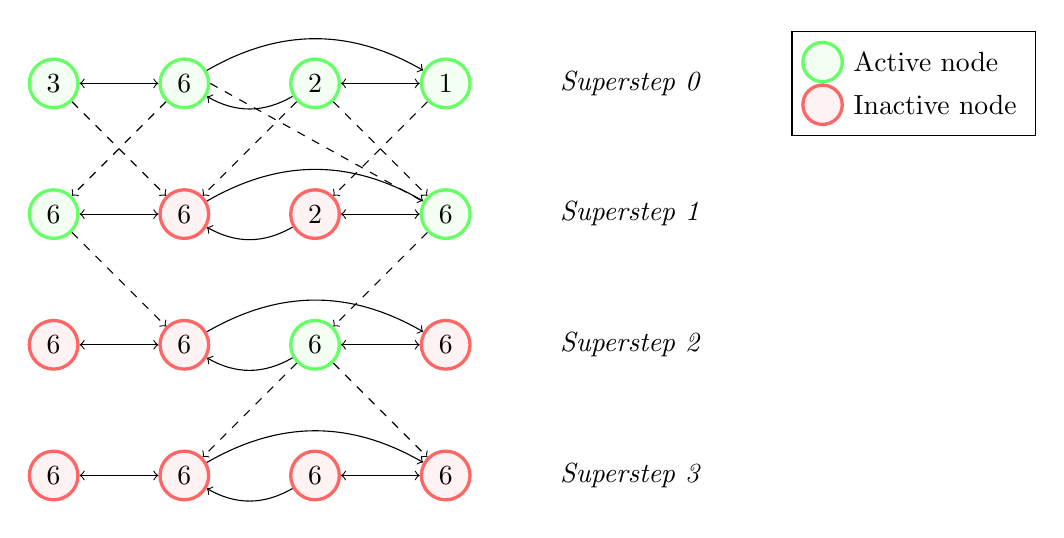
\begin{tikzpicture}[
        activenode/.style={circle, draw=green!60, fill=green!5, very thick, minimum size=5mm},
        inactivenode/.style={circle, draw=red!60, fill=red!5, very thick, minimum size=5mm},
    ]
    %Nodes: Superstep 0
    \node[activenode]   (super0_left)                                    {3};
    \node[activenode]   (super0_centerleft) [right=of super0_left]       {6};
    \node[activenode]   (super0_centeright) [right=of super0_centerleft] {2};
    \node[activenode]   (super0_right)      [right=of super0_centeright] {1};

    \node (super0) [right=of super0_right] {\textit{Superstep 0}};

    %Nodes: Superstep 1
    \node[activenode]     (super1_left)       [below=of super0_left]       {6};
    \node[inactivenode]   (super1_centerleft) [below=of super0_centerleft] {6};
    \node[inactivenode]   (super1_centeright) [below=of super0_centeright] {2};
    \node[activenode]     (super1_right)      [below=of super0_right]      {6};

    \node [right=of super1_right] {\textit{Superstep 1}};

    %Nodes: Superstep 2
    \node[inactivenode]   (super2_left)       [below=of super1_left]       {6};
    \node[inactivenode]   (super2_centerleft) [below=of super1_centerleft] {6};
    \node[activenode]     (super2_centeright) [below=of super1_centeright] {6};
    \node[inactivenode]   (super2_right)      [below=of super1_right]      {6};

    \node [right=of super2_right] {\textit{Superstep 2}};

    %Nodes: Superstep 3
    \node[inactivenode]   (super3_left)       [below=of super2_left]       {6};
    \node[inactivenode]   (super3_centerleft) [below=of super2_centerleft] {6};
    \node[inactivenode]   (super3_centeright) [below=of super2_centeright] {6};
    \node[inactivenode]   (super3_right)      [below=of super2_right]      {6};

    \node [right=of super3_right] {\textit{Superstep 3}};

    %Dashed lines: connections between nodes
    \path[dashed,-to] (super0_left) edge node {} (super1_centerleft);
    \path[dashed,-to] (super0_centerleft) edge node {} (super1_left);
    \path[dashed,-] (super0_centerleft.east) edge node {} (super1_right);
    \path[dashed,-to] (super0_centeright) edge node {} (super1_centerleft);
    \path[dashed,-to] (super0_centeright) edge node {} (super1_right);
    \path[dashed,-to] (super0_right) edge node {} (super1_centeright);

    \path[dashed,-to] (super1_left) edge node {} (super2_centerleft);
    \path[dashed,-to] (super1_right) edge node {} (super2_centeright);

    \path[dashed,-to] (super2_centeright) edge node {} (super3_centerleft);
    \path[dashed,-to] (super2_centeright) edge node {} (super3_right);

    %Lines: connections between nodes
    \path[to-to] (super0_left)       edge             node {} (super0_centerleft);
    \path[-to]   (super0_centerleft) edge[bend left]  node {} (super0_right);
    \path[to-]   (super0_centerleft) edge[bend right] node {} (super0_centeright);
    \path[to-to] (super0_centeright) edge             node {} (super0_right);

    \path[to-to] (super1_left)       edge             node {} (super1_centerleft);
    \path[-to]   (super1_centerleft) edge[bend left]  node {} (super1_right);
    \path[to-]   (super1_centerleft) edge[bend right] node {} (super1_centeright);
    \path[to-to] (super1_centeright) edge             node {} (super1_right);

    \path[to-to] (super2_left)       edge             node {} (super2_centerleft);
    \path[-to]   (super2_centerleft) edge[bend left]  node {} (super2_right);
    \path[to-]   (super2_centerleft) edge[bend right] node {} (super2_centeright);
    \path[to-to] (super2_centeright) edge             node {} (super2_right);

    \path[to-to] (super3_left)       edge             node {} (super3_centerleft);
    \path[-to]   (super3_centerleft) edge[bend left]  node {} (super3_right);
    \path[to-]   (super3_centerleft) edge[bend right] node {} (super3_centeright);
    \path[to-to] (super3_centeright) edge             node {} (super3_right);

    %Legend: active and inactive nodes
    \matrix [draw,below left] [right=of super0] {
        \node [activenode,label=right:Active node] {};     \\
        \node [inactivenode,label=right:Inactive node] {}; \\
    };
\end{tikzpicture}
\end{document}